\chapter{Conclusioni}
\label{cha:conclusioni}

In quest'ultimo capitolo commenterò gli obiettivi raggiunti e le funzionalità implementate. Parlerò del percorso di formazione che mi ha aiutato nella progettazione e creazione del bot, dello stato attuale del lavoro e, infine, trarrò alcune considerazioni soggettive. 

\section{Raggiungimento degli obiettivi}

Gli obiettivi prefissati per questo progetto sono stati raggiunti. Tutte le fasi necessarie alla realizzazione del bot sono state eseguite. In particolare, sono partito da una prima fase di analisi dei requisiti, per poi passare alla progettazione tecnica dei vari aspetti del bot e, infine, allo sviluppo vero e proprio. Al momento attuale, il bot risulta funzionante e dalla sua pubblicazione è stato utilizzato da circa 500 utenti. 

\subsection{Funzionalità del bot}

Come descritto nel capitolo \ref{cha:analisi_progettazione}, le funzionalità sviluppate sono: 
\begin{itemize}
\item consultare gli orari di autobus urbani e extraurbani;
\item consultare gli orari delle ferrovie Brennero, Valsugana e Trento-Mezzana;
\item visualizzare su una mappa dove si trova un autobus in tempo reale e avere la possibilità di seguirlo durante il suo percorso;
\item visualizzare il ritardo e l'ultima posizione conosciuta dei mezzi;
\item visualizzare il numero di posti liberi nei parcheggi dei comuni di Trento e Rovereto;
\item sapere la disponibilità di bici elettriche presenti nelle stazioni di ricarica;
\item salvare le fermate e linee preferite per una consultazione di orari e ritardi molto più veloce;
\item rimanere informati su eventuali scioperi, variazioni di percorso, fermate sospese.
\end{itemize}

\section{Sviluppi futuri}

\begin{wrapfigure}{r}{0.38\textwidth}
\centering
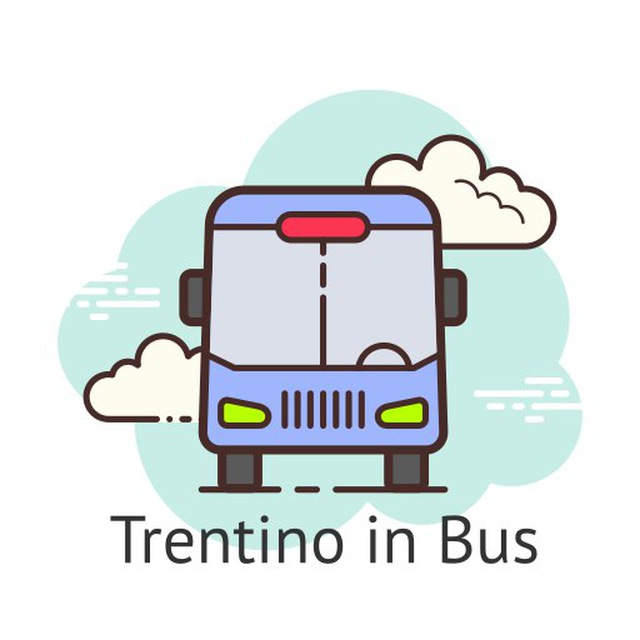
\includegraphics[scale=0.2]{TrentinoInBus.jpg}
\caption{Logo TrentinoInBus}
\label{fig:trentino_in_bus}
\end{wrapfigure}

Dopo aver analizzato alcuni dei migliori servizi sul mercato e aver eseguito una piccola fase di valutazione del bot, ho eseguito un brainstorming su come poterlo migliorare ed espandere. 

Sicuramente sarebbe interessante orientarsi verso una soluzione \textit{MaaS}, aggiungendo informazioni sui servizi in sharing e di micro-mobilità, e permettendo agli utenti di organizzare i propri spostamenti fornendo varie opzioni. Se ci si orienta verso questa soluzione sarebbe poi necessario implementare un sistema di pagamento direttamente nel bot. Fortunatamente Telegram, tramite le sue \textit{Bot Payments API}, mette a disposizione delle API per ricevere pagamenti per beni e servizi dagli utenti. Telegram e lo sviluppatore del bot non processano nessun pagamento e non accedono a nessuna informazione sensibile, ma fanno affidamento ai più famosi provider di pagamento come \textit{Stripe}.

La funzionalità di monitoraggio dei parcheggi si potrebbe anch'essa migliorare aggiungendo la possibilità di gestire e pagare la sosta direttamente dal bot e permettendo di trovare i parcheggi ottimali in base alla propria destinazione.

\subsection{Scalabilità, replicabilità, problemi e limitazioni}
\label{sec:scalabilita}
Dal punto di vista tecnico, il bot, essendo stato sviluppato utilizzando tecnologie fortemente scalabili, non presenterà alcun problema nel caso di un incremento delle funzionalità o degli utenti. Infatti, \textit{NodeJs} fornisce meccanismi di \textit{Load Balancing} e MongoDB permette di essere scalabile sia orizzontalmente, attraverso lo \textit{sharding}, che verticalmente, aggiungendo più CPU e RAM.


Il bot Telegram  potrebbe potenzialmente essere replicato ed utilizzato in ogni luogo del mondo facendo dei piccoli adattamenti e integrando le API esterne necessarie al suo funzionamento.


I problemi principali, al momento, sono connessi alla ricerca e integrazione di API pubbliche. Risulta necessario trovare delle API che permettano il supporto a più zone, quindi non solo in Trentino, e che forniscano la possibilità di integrare i pagamenti per l'acquisto di biglietti o delle soste. Fortunatamente, le API di \textit{ViaggiaTreno} utilizzate al momento nel bot, in riferimento alle informazioni sulle ferrovie, possono essere estese all'utilizzo sull'intero territorio nazionale. 

Visto il progetto di espandere il servizio, telegram, e in particolare le funzionalità offerte dai bot, potrebbero risultare limitanti andando a rendere anche più difficile l'utilizzo da parte dell'utente. Inoltre, se l'espansione riguarderà i territori coperti dal bot potrebbe risultare utile creare una serie di bot, uno per zona, con tutte le funzionalità. Questo permetterà di mantenere un'interfaccia chiara e non appesantita da troppe azioni per l'utente. 

Infine, il nome del bot, \textit{@TrentinoInBusBot}, risulta essere riduttivo e poco rappresentativo rispetto alle tante funzionalità già presenti. Potrebbe quindi essere utile rinominarlo con un nome più emblematico rispetto alle tante possibilità offerte. 

\section{Formazione}

Per la creazione di questo bot, lo studio delle tecnologie è stato individuale. Per la fase di analisi alcuni corsi universitari, come \textit{Ingegneria del software 1 e 2} e \textit{Human-Computer Interaction}, sono risultati fondamentali per la buona riuscita. 
Grazie all'esperienza di tirocinio formativo,  presso l'azienda \textit{Zupit}, dove ho potuto approfondire varie caratteristiche dello sviluppo web, è stato più semplice e veloce imparare nuovi linguaggi e tecnologie.

\section{Conclusioni soggettive}

Il lavoro di progettazione e implementazione mi hanno dato l'opportunità di migliorare ulteriormente la preparazione offerta dal corso di studi. Lo sviluppo di un progetto pratico sarà sicuramente utile ai fini dei futuri impegni lavorativi e come aggiunta al proprio portfolio personale. 

Grazie all'esperienza di tirocinio, ho potuto seguire per intero il processo di realizzazione di alcuni progetti, questo mi ha aiutato a migliorare la gestione delle possibili problematiche legate a ciascuna fase del mio progetto, con maggiore attenzione e prontezza. 